
%%%%%%
%
% $Autor: Manoj Selvaraju $
% $Datum: 2024-01-05 11:15:45Z $
% $Pfad: githubtemplate/Template/report/rename.tex $
% $Version: 4620 $
%
%
% !TeX encoding = utf8
% !TeX root = Rename
% !TeX TXS-program:bibliography = txs:///bibtex
%
%%%%%%

\chapter{TensorFlow Lite}

\section{TensorFlow}
\label{sec:Tensor_Flow}

TensorFlow is a free and open-source software library, tool or a platform for machine learning and artificial intelligence, developed by the Google Brain team. It can be used across a range of tasks but has a particular focus on training and inference of deep neural networks.  \cite{tensorflowWiki:2024}

TensorFlow uses dataflow graphs to represent computation, shared state, and the operations that mutate that state. It can train and run deep neural networks for applications such as handwritten digit classification, image recognition, word embeddings, recurrent neural networks, sequence-to-sequence models for machine translation, natural language processing, and PDE (partial differential equation) based simulations. TensorFlow maps the nodes of a dataflow graph across many machines in a cluster and within a machine across multiple computational devices, including multicore CPUs, general-purpose GPUs, and custom-designed ASICs known as Tensor Processing Units (TPUs). \cite{tensorflow:2024} \cite{abadi2016tensorflow}
%It enables developers to experiment with novel optimizations and training algorithms. Several Google services use TensorFlow in production, and it has become widely used for machine learning research since its release as an open-source project.  

\begin{comment}
\section{TensorFlow Use Case}

Google search engine also based on Tensor flow AI application, e.g; when a user type "a" in the google search bar, the search engine predict the most suitable complete word to select, or it may be predicts depends upon the previous search on the same system by the user too. It can be used across a range of tasks but has a particular focus on training and inference of deep neural networks. Tensor flow has a various collection of workflows to develop and train the model using Python and Javascripts programming languages, after training the model we can deploy the model on the Cloud or also on any device for making edge computing application no matter which language use in the device. It is obvious that, the most important part in every Machine learning application is to train the ML model, so the model will apply in real time condition and take the decision without any human intervention as the human normally make.
\end{comment}

\section{pyTorch}
\label{sec:pyTorch}
PyTorch is an open-source machine learning library, based on the Torch library, developed by Facebook's AI Research lab. Although Pytorch is launched after TensorFlow, it has quickly gained popularity due to its ease of customization. Unlike static computation graphs, PyTorch allows users to define and manipulate the graph dynamically during runtime, which makes debugging and model development more easier. This flexibility is highly beneficial for tasks such as natural language processing, computer vision, and reinforcement learning. PyTorch supports both CPU and GPU computation, offering seamless acceleration using CUDA for high-performance GPU computations. PyTorch's framework is also deeply integrated with Python, making it a preferred choice for researchers and developers. \cite{pytorchWiki:2024} \cite{pytorch:2024}
\begin{comment}
PyTorch provides two key features
\begin{itemize}
	\item Tensor computation (similar to NumPy) with strong GPU acceleration
	\item Deep neural networks built on a dynamic autograd system, which tracks computations at runtime for automatic differentiation.
\end{itemize}
\end{comment}

\section{JAX}
\label{sec:JAX}
JAX is a open source machine learning library developed by Google that is designed for high-performance numerical computing and automatic differentiation. Unlike traditional deep learning libraries, JAX is built around NumPy and works with various existing frameworks such as TensorFlow and PyTorch with automatic differentiation and it is highly optimised to run on CPUs, GPUs and TPUs. \cite{jax:2024}

\section{Keras}
\label{sec:Keras}
Keras is a high-level deep learning Application Programming Interface (API) written in Python for fast experimentation with neural networks. Initially developed as an independent library, Keras is now tightly integrated into TensorFlow and serves as its official high-level API. Now Keras 3, multi-framework deep learning API is a full rewrite of Keras that enables you to run your Keras workflows on top of either JAX, TensorFlow, or PyTorch, and that unlocks brand new large-scale model training and deployment capabilities. Keras is powerful and can handle a wide variety of tasks such as image classification, natural language processing, and reinforcement learning. It supports both CPU and GPU computation and can be deployed on mobile and web applications. \cite{keras:2024}

\section{TensorFlow Lite}
\label{sec:TensorFlow Lite}

Tensorflow Lite is an optimised environment of TensorFlow models, which is specifically designed for mobile and edge devices, allowing machine learning models to run efficiently on smartphones, embedded systems and other devices with limited computational resources.
Essentially it consists of two components, the model converter, which converts pre-trained TensorFlow models into optimised TensorFlow Lite models and the Interpreter, which enables efficient execution on end devices. \cite{tensorflow_lite:2024} 
%It's primary focus on reducing the size of the existing models and to reduce the latency on low powered devices.
\medskip
TensorFlow Lite has now been officially renamed to LiteRT. Now, LiteRT (formerly TensorFlow Lite) grown beyond its TensorFlow roots to support models from other frameworks like PyTorch, JAX, and Keras. LiteRT continues to serve as the optimized environment for running AI models on mobile devices, embedded systems, and other edge devices, focusing on reducing model size, latency, and energy consumption.
The name change reflects how this high-performance runtime has evolved beyond supporting only TensorFlow models to also include models from other frameworks like PyTorch, JAX, and Keras. LiteRT continues to serve as the optimized environment for running AI models on mobile devices, embedded systems, and other edge devices, focusing on reducing model size, latency, and energy consumption. \cite{9to5google_LiteRT:2024}

\section{Why TensorFlow Lite?}
Often the trained models are not to be used on the PC on which they were trained,but on mobile devices such as mobile phones or microcontrollers or other embedded systems. However, limited computing and storage capacities are available there. TensorFlow Lite is a whole framework that allows the conversion of models into a special format and their optimization in terms of size and speed, so that the models can then be run with TensorFlow Lite interpreters on mobile, embedded and IoT devices. \cite{tfl_guide:2024}

However, you cannot train a model directly with TensorFlow Lite, it must first be created with TensorFlow, then you must convert the model from a TensorFlow file to a TensorFlow Lite file using the TensorFlow Lite converter. The reason is that TensorFlow models usually calculate in 32-bit floating point numbers for the neural networks. The weights can assume very small values close to zero. Therefore, the models cannot be run on systems that cannot calculate with long floating point numbers, but only with 8-bit integers. This is especially the case with small AI processors, on which only a few transistors can be accommodated due to size and power consumption. Therefore, the neural network must undergo a transformation, in which long floating-point numbers with varying precision over the representable range of values– floating-point numbers represent the range of numbers around the zero point much more finely than very large or small values– become short integers with constant precision in a limited range of values. \cite{coral_ai}


\section{Working Procedure of TensorFlow Lite}

TensorFlow Lite workflow consists of four steps as illustrated in the figure ~\ref{TensorLiteWorkflow} Here’s how TensorFlow Lite works:  \cite{tensorflow_lite:2024}

\begin{enumerate}
	\item Model Creation
	\item Model Conversion
	\item Model Deployment
	\item Model Optimization
\end{enumerate}

\begin{figure}[h]
	\centering
	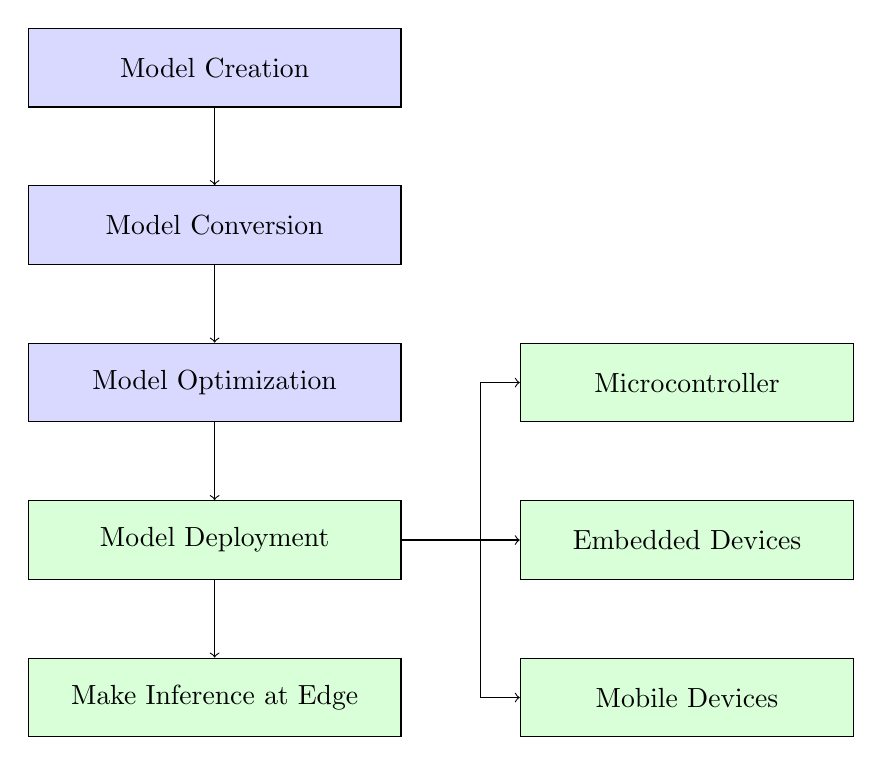
\begin{tikzpicture}[node distance=2cm, auto]
		% Node style
		\tikzstyle{block} = [rectangle, draw=black, fill=blue!15, text width=4.5cm, text centered, minimum height=1cm]
		
		% Nodes
		\node[block] (creation) {Model Creation};
		\node[block, below of=creation] (conversion) {Model Conversion};
		\node[block, below of=conversion] (optimization) {Model Optimization};
		\node[block, draw=black, fill=green!15, below of=optimization] (deployment) {Model Deployment};
		\node[block, draw=black, fill=green!15, below of=deployment] (inference) {Make Inference at Edge};
		
		\node[block, draw=black, fill=green!15, right of=deployment, xshift=4cm, yshift=2cm, text width=4cm] (microcontroller) {Microcontroller};
		\node[block, draw=black, fill=green!15, right of=deployment, xshift=4cm, text width=4cm] (embedded) {Embedded Devices};
		\node[block, draw=black, fill=green!15, right of=deployment, xshift=4cm, yshift=-2cm, text width=4cm] (mobile) {Mobile Devices};
		
		% Arrows
		\draw[->] (creation) -- (conversion);
		\draw[->] (conversion) -- (optimization);
		\draw[->] (optimization) -- (deployment);
		\draw[->] (deployment) -- (inference);
		\draw[->] (deployment.east) -- ++(1,0) |- (microcontroller.west);
		\draw[->] (deployment.east) -- (embedded.west);
		\draw[->] (deployment.east) -- ++(1,0) |- (mobile.west);
	\end{tikzpicture}
	\caption{TensorLite Workflow}
	\label{TensorLiteWorkflow}
\end{figure}


\subsection{Model Creation and Training}
The first step involves creating and training a machine learning model using TensorFlow. 
\\TensorFlow Lite uses TensorFlow models converted into a smaller, more efficient machine learning (ML) model format. You can use pre-trained models with TensorFlow Lite, modify existing models, or build your own TensorFlow models and then convert them to TensorFlow Lite format. TensorFlow Lite models can perform almost any task a regular TensorFlow model can do: object detection, natural language processing, pattern recognition, and more using a wide range of input data including images, video, audio, and text. \cite{tensorflow_lite:2024}

The listing ~\ref{lst:modelCreationTraining} explains the workflow of creating and training a simple neural network model using TensorFlow's Keras API. Also it simplifies a simple example of image classification involving steps in preparing data from MNIST dataset, building, training, evaluating the model for further conversion to TensorFlow Lite format. \cite{tfModelCreationKeras:2024}

\begin{code}
\begin{lstlisting}[language=Python, caption={Model Creation and Training Example Using TensorFlow}, label={lst:modelCreationTraining}]
	import tensorflow as tf
	from tensorflow.keras.models import Sequential
	from tensorflow.keras.layers import Dense, Flatten
	from tensorflow.keras.optimizers import Adam
	
	# Load the MNIST dataset
	mnist = tf.keras.datasets.mnist
	(x_train, y_train), (x_test, y_test) = mnist.load_data()
	
	# Normalize the images to the range [0, 1]
	x_train, x_test = x_train / 255.0, x_test / 255.0
	
	# Define a simple Sequential model
	model = Sequential([
	Flatten(input_shape=(28, 28)),  # Flatten the 28x28 images into a 1D array of 784 elements
	Dense(128, activation='relu'),  # Hidden layer with 128 neurons and ReLU activation
	Dense(10, activation='softmax') # Output layer with 10 neurons for classification
	])
	
	# Compile the model with an optimizer, loss function, and metric
	model.compile(optimizer=Adam(),
	loss='sparse_categorical_crossentropy',
	metrics=['accuracy'])
	
	# Train the model on the training data
	model.fit(x_train, y_train, epochs=5, validation_data=(x_test, y_test))
	
	# Evaluate the model on the test data
	test_loss, test_acc = model.evaluate(x_test, y_test, verbose=2)
	print(f'\nTest accuracy: {test_acc:.4f}')
	
	# Save the trained model as a SavedModel format (for future conversion to TFLite)
	model.save('saved_model/my_mnist_model')
\end{lstlisting}
\end{code}

\subsection{Model Conversion}
\label{subsec:model_conversion}
Once the model is trained, it needs to be converted into a TensorFlow Lite model. The TensorFlow Lite converter takes a TensorFlow model and generates a TensorFlow Lite model, an optimized FlatBuffer format identified by the file extension \FILE{.tflite}. \cite{tensorflowModelConversion:2024}

The model conversion can be done using the Python API or the Command
line tool
\begin{itemize}
	\item Command-line Tool: \SHELL{tflite convert}, this allows you to integrate the conversion into your development pipeline, apply optimizations, add metadata and many other tasks that simplify the conversion process.
	\item Python API: \SHELL{tf.lite.TFLiteConverter}, this only supports basic model conversion.
\end{itemize}

The process involves following steps:
\begin{itemize}
	\item \textbf{Select the Model}: The converter accepts the following input model formats.
	\begin{itemize}
		\item \FILE{SavedModel}: A TensorFlow model saved as a set of files on disk.
		\SHELL{tf.lite.TFLiteConverter.from\_saved\_model(model)}
		\item \FILE{Keras model}: A model created using the high level Keras API.
		\SHELL{tf.lite.TFLiteConverter.from\_keras\_model(model)}
		\item \FILE{Keras H5 format}: A light-weight alternative to SavedModel format supported by Keras API.
		\SHELL{tf.lite.TFLiteConverter.from\_keras\_model(model\_loaded\_from\_model.h5)}
		\item \FILE{Models built from concrete functions}: A model created using the low level TensorFlow API.
		\SHELL{tf.lite.TFLiteConverter.from\_concrete\_functions([func], model)}
	\end{itemize}
	The listing ~\ref{lst:modelConversionCode} provides the APIs for the above mentioned models. \cite{tflConversionAPI:2024}
	
\begin{code}
	% Include a specific range of lines from the Python file for Model Conversion
	\lstinputlisting[
	language=Python, 
	firstline=1, 
	lastline=22, 
	caption={Python Code for Converting Models to .tflite}, 
	label={lst:modelConversionCode}
	]{../Code/TensorFlowLite/ModelConversionCode.py}
\end{code}
	
	\item \textbf{Optimize the Model}: During conversion, various optimization techniques can be applied to make the model more efficient. These includes quantization, Pruning, Clustering.
\end{itemize}

The goal of these optimizations is to make the model smaller and faster while maintaining accuracy.

\subsection{Model Deployment}
After converting the model to a file \FILE{.tflite}, it can be deployed on a variety of devices including mobile phones, embedded systems, and microcontrollers. TensorFlow Lite supports deployment on both Android and iOS platforms, as well as other systems like Arduino.

\subsection{Running Inference}
The term inference refers to the process of executing a TensorFlow Lite model on-device in order to make predictions based on input data. To perform an inference with a TensorFlow Lite model, you must run it through an interpreter. The TensorFlow Lite interpreter is designed to be lean and fast. The interpreter uses a static graph ordering and a custom (less-dynamic) memory allocator to ensure minimal load, initialization, and execution latency. \cite{tensorflowLiteInference:2024} \cite{GoogleAIEdge:2024}

Here’s the typical process:

\begin{itemize}
	\item \textbf{Load the Model}: The TensorFlow Lite model file \FILE{.tflite} is loaded into the memory, which contains the model's execution graph. 
	The listing \ref{lst:modelLoading} provides the code for Loading and Validating a TensorFlow Lite Model for Microcontroller.

	\begin{code}
	% Include a Model loading line code from the C++ file
	\lstinputlisting[language=C++, firstline=1, lastline=17, label={lst:modelLoading}, caption={Loading and Validating a TensorFlow Lite Model for Microcontroller}]{../Code/TensorFlowLite/InferenceLoadingModel.cpp}
	\end{code}
	
	\item \textbf{Allocate Tensors}: Build an Interpreter based on an existing model, that is allocating memory for the input and output tensors. 
	The listing \ref{lst:AllocateTensor} provides the reference code for Allocating Tensors for TensorFlow Lite Model Execution on Microcontroller.

	\begin{code}
	%  
	\lstinputlisting[language=C++, firstline=1, lastline=17, label={lst:AllocateTensor}, caption={Allocating Tensors for TensorFlow Lite Model Execution}]{../Code/TensorFlowLite/InferenceAllocateTensor.cpp}
	\end{code}

	\item \textbf{Set Input Data}: Set input tensor values (Optionally resize input tensors if the predefined sizes are not desired) and fed into the model. 
	The listing \ref{lst:InputData} gives the reference code for setting Input Data for TensorFlow Lite Inference on a Microcontroller.
	\begin{code}
		%  
		\lstinputlisting[language=C++, firstline=1, lastline=17, label={lst:InputData}, caption={Setting Input Data for TensorFlow Lite Inference}]{../Code/TensorFlowLite/InferenceInputData.cpp}
	\end{code}
	
	\item \textbf{Invoke the Interpreter}: The interpreter runs the model with the input data to produce the output. 
	The listing \ref{lst:InvokeInterpreter} gives the reference code for invoking TensorFlow Lite Interpreter to perform Inference on a Microcontroller.
	\begin{code}
		% 
		\lstinputlisting[language=C++, firstline=1, lastline=17, label={lst:InvokeInterpreter}, caption={Invoking TensorFlow Lite Interpreter to perform Inference on a Microcontroller}]{../Code/TensorFlowLite/InferenceRunning.cpp}
	\end{code}
	
	\item \textbf{Get Output Data}: The output data is extracted and post-processed to get the final predictions. 
	The listing \ref{lst:OutputData} gives the reference code Extracting and Processing Output Data from a TensorFlow Lite Model																																 on a Microcontroller
	\begin{code}
		% 
		\lstinputlisting[language=C++, firstline=1, lastline=5, label={lst:OutputData}, caption={Extracting and Processing Output Data from a TensorFlow Lite Model}]{../Code/TensorFlowLite/InferenceOutputData.cpp}
	\end{code}
	
\end{itemize}

% Include a specific range of lines from the Python file for InterfaceCode
%\lstinputlisting[language=Python, firstline=1, %lastline=17]{../Code/TensorFlowLite/InterfaceCode.py}

\subsubsection{Tensors in TensorFlow Lite}
In TensorFlow Lite, a tensor is a multi-dimensional array that represents the basic data structure used by the library. Just like a vector is a one-dimensional array and a matrix is a two-dimensional array, a tensor can be n-dimensional. Tensors can have different shapes and data types, and they are used for both input and output of the model. \cite{tensorflowLiteInference:2024}
\begin{comment}
Here's a brief overview of tensors

\subsection{Shape} 
The shape of a tensor defines the number of elements in each dimension. For example, a tensor with shape [2, 3, 4] has 2 elements in the first dimension, 3 elements in the second dimension, and 4 elements in the third dimension.

\subsection{Data Type}
Tensors can contain different types of data, such as integers, floating-point numbers, or strings. The data type is specified when the tensor is created.

\subsection{Usage in TensorFlow Lite}
\begin{itemize}
	\item \textbf{Input Tensors}: These are used to feed the input data into the model. The input tensor shape and data type must match what the model expects.
	\item \textbf{Output Tensors}: These store the results produced by the model after running inference. The output tensor shape and data type depend on the model's architecture and the specific task it performs.
\end{itemize}

\subsection{Tensor Examples}
\begin{itemize}
	\item If a model expects an input image of size 224x224 with 3 color channels (RGB), the input tensor shape might be [1, 224, 224, 3], where 1 represents the batch size. After running inference, the output might be a tensor of shape [1, 1000] if the model outputs probabilities for 1000 different classes.
	\item If an object detection model processes an input image of size 300x300 with 3 color channels (RGB), the input tensor shape might be [1, 300, 300, 3]. The output tensor might include bounding boxes, with a shape of [1, 10, 4] where 10 represents the number of detected objects and 4 represents the coordinates of each bounding box.
\end{itemize}
\end{comment}

\chapter{Comprehensive TensorFlow Lite Usage Methodologies}
This section broadly covers the various contexts in which TensorFlow Lite is used, including its role in microcontrollers (Arduino), as a tool for model conversion and optimization and as a library path in larger projects.

\section{TensorFlow Lite as a Library for Arduino}
TensorFlow Lite for Microcontrollers is a version of TensorFlow Lite designed to run machine learning models on microcontroller devices, such as those based on the Arduino platform. This library is highly optimized to work within the constraints of small devices with limited resources (e.g., very low memory and processing power). \cite{tensorflowblog:2024}

\subsection{Usage and Integration}

When you use TensorFlow Lite on an Arduino, you typically include the TensorFlow Lite Micro library in your Arduino IDE. This allows you to write programs that can perform tasks like speech recognition, gesture detection, or even basic image classification directly on the Arduino. The library is optimized to run on devices with very limited resources, such as minimal RAM and processing power. 
The library is installed into the Arduino development environment, and you can include it in your projects by adding the appropriate headers and linking against the library when compiling your code. This allows your Arduino sketches to utilize TensorFlow Lite models. \cite{tensorflowblog:2024}


\subsection{TensorFlow Lite Micro Arduino Example}
TensorFlow Lite Micro Library for Arduino repository contains examples needed to use Tensorflow Lite Micro on an Arduino. To implement, first clone the TensorFlow Lite Micro Arduino Examples repository from GitHub into a local directory called \PATH{Arduino\_TensorFlowLite}. This repository contains examples for using TensorFlow Lite on microcontrollers like Arduino for various machine learning tasks, such as image classification and voice recognition, optimized for low-power devices like Arduino. \cite{tensorflowblog:2024}. 
\\Run the command \SHELL{git clone https://github.com/tensorflow/tflite-micro-arduino-examples} as per figure ~\ref{Clone}

\begin{figure}
	\begin{center}
		\includegraphics[width=0.7\linewidth]{Images/TensorFlowLite/TFLiteMicro.png}
		\caption{TFlite Micro github Cloning to local repository}
		\label{Clone}
	\end{center}
\end{figure}

Once the library is installed, Open Arduino IDE, go to \SHELL{Files > Examples > Arduino\_TensorFlowLite > hello\_world} as shown in figure ~\ref{TFLlib}.

\begin{figure}
	\begin{center}
		\includegraphics[width=0.7\linewidth]{Images/TensorFlowLite/helloWorld.png}
		\caption{TensorFlow Lite as a Library for Arduino}
		\label{TFLlib}
	\end{center}
\end{figure}

This example program, hello\_world, is designed to replicate a sine wave using a TensorFlow Lite model. The model generates a pattern that varies the brightness of the built-in LED on an Arduino in a pattern similar to the last predicted sine value. Since the value ranges from -1 to 1, we could represent 0 with a fully off LED, -1 and 1 with a fully lit LED, and all intermediate values with a partially dimmed LED. As the program loops, making inferences, the LED fades in and out repeatedly. To dim our built-in LED, we use a technique called pulse width modulation (PWM). If we turn an output pin on and off extremely quickly, the output voltage of the pin is set to a factor of ratio the time spend between on and off states. If the pin spends half of the time in each state, its output voltage will be half of its maximum (50 percent). 
With the \PYTHON{constantkInferencesPerCycle} the number of inferences performed over a full sine cycle can be varied. Since an inference takes a certain amount of time, by setting the \PYTHON{constantkInferencesPerCycle}, can be set how quickly the LED fades out. \cite{tensorflowblog:2024}

First, we include some header files in the source code (refer ~\ref{lst:helloworld}). These headers include the essential TensorFlow Lite for Microcontrollers (TFLM) files, allowing the model and interpreter to function.

The global variables define pointers to the model, interpreter, input/output tensors, and a tensor arena for storing intermediate data.
The \PYTHON{setup()} function initializes the TensorFlow Lite model and sets up the necessary components such as Model Initialization, Operations Resolver \PYTHON{AllOpsResolver} object used to load all necessary operations for the model, Interpreter setup, Tensor Allocation and Tensor Pointers.

The \PYTHON{loop()} function performs continuous inferences using the sine wave model
The loop function first calculates the current x-value based on \PYTHON{inference\_count}, then quantizes the x-value to an integer format, reducing memory and computation requirements. It executes the model inference, updating the output tensor with the result. Following this, it dequantizes the output back to floating-point, generating the sine wave value y. The \PYTHON{HandleOutput()} function is used to update the LED based on the sine wave pattern. Finally, it increments the \PYTHON{inference\_count} and resets it after completing a full sine wave cycle.


\begin{code}
	% Include a specific range of lines from the Python file for Model Conversion
	\lstinputlisting[
	language=C++, 
	firstline=16, 
	lastline=115, 
	caption={Hello World Program}, 
	label={lst:helloworld}
	]{../Code/TensorFlowLite/SineWaveLED/SineWaveLED.ino}
\end{code}

To run the example, connect your Arduino device via USB. Make sure the correct device type is selected in the Board drop-down list in the Tools menu, \SHELL{Tools > Board}. If the device not appears in the list, go to \SHELL{Tools > Board > Board Manager} and in the window appears, install the latest version of the supported board package. Then make sure the device port is selected as shown in the figure ~\ref{BoardPort} \cite{tensorflowblog:2024}.

\begin{figure}
	\begin{center}
		\includegraphics[width=0.7\linewidth]{Images/TensorFlowLite/BoardPortSelection.png}
		\caption{Board and Port selection}
		\label{BoardPort}
	\end{center}
\end{figure}

Then finally, in the Arduino window, click the Upload button to compile the code and upload it to your Arduino device.
After the upload has completed successfully, you should see the LED on your Arduino board start to either fade in and out or blink on and off, depending on whether the pin it is connected to supports PWM.

This example demonstrates a simple end-to-end workflow for using TensorFlow Lite as a Library for Arduino Microcontrollers by training and deploying a model to Arduino.

\section{TensorFlow Lite as a Library Path}

In software development, TensorFlow Lite as a library path refers to integrating TFLite as a reusable resource into a broader project, whether it's a mobile application, embedded system, or even a desktop application. The concept of a "library path" in this context refers to how TFLite’s library is organized, included, and linked within a project's build system, such as CMake, Bazel, or Makefiles, to streamline access across multiple components \cite{tensorflowlitemicro:2024}.

When TensorFlow Lite is treated as an external library, it provides a centralized resource that enables different parts of a project to access TFLite's models, functions, and interpreter without duplicating or moving source files. 

\subsection{Usage and Integration:}

In building an application with TensorFlow Lite, ensuring that the development environment has access to the TFLite libraries is essential for linking during the build process. This often involves specifying paths in the build configuration files (such as CMakeLists.txt or BUILD files) to include TensorFlow Lite's headers and binary files \cite{Google_TFLite_ARM:2024}. A "library path" refers to the directory where TensorFlow Lite binaries, headers, and other resources are stored. This path is specified in the build configuration so that the compiler and linker can locate TensorFlow Lite components seamlessly.

In large project setup, TensorFlow Lite enables inference on pre-trained models, providing localized AI functionalities directly on the device. By setting TFLite up as a library path, this approach allows each application component to perform machine learning tasks independently, with consistent access to TFLite’s resources.

\subsubsection{Directory Structure Example}
For an organized project, here’s an example directory structure ~\ref{Directory} that illustrates how TensorFlow Lite might be set up as a library path,

\begin{figure}[h]
	\centering
\begin{tikzpicture}[
	every node/.style={font=\ttfamily, anchor=west},
	level distance=10mm,
	sibling distance=0mm,
	edge from parent path={(\tikzparentnode.south) |- (\tikzchildnode.west)}
	]
	
	\node {MyProject}
	child { node [xshift=5mm] {CMakeLists.txt} }
	child [yshift=-10mm] { node [xshift=5mm] {libs}
		child { node [xshift=5mm] {tensorflow\_lite}
			child { node [xshift=5mm] {include}
				child { node [xshift=5mm] {tensorflow}
					child { node [xshift=5mm] {lite}
						child { node [xshift=5mm] {micro}
							child [yshift=-10mm] { node [xshift=5mm] {all\_ops\_resolver.h} }
							child [yshift=-20mm] { node [xshift=5mm] {micro\_interpreter.h} }
							child [yshift=-30mm] { node [xshift=5mm] {kernels} }
							child [yshift=-40mm] { node [xshift=5mm] {...} }
						}
					}
				}
			}
			child [yshift=-80mm] { node [xshift=5mm] {lib}
				child { node [xshift=5mm] {libtensorflowlite.a} }
			}
		}
	}
	child [yshift=-120mm] { node [xshift=5mm] {src}
		child { node [xshift=5mm] {component1}
			child [yshift=-10mm] { node [xshift=5mm] {component1.cpp} }
			child [yshift=-20mm] { node [xshift=5mm] {component1.h} }
		}
		child [yshift=-40mm] { node [xshift=5mm] {component2} 
			child [yshift=-10mm] { node [xshift=5mm] {component2.cpp} }
			child [yshift=-20mm] { node [xshift=5mm] {component2.h} }
		}
		child [yshift=-80mm] { node [xshift=5mm] {main.cpp} }
	};
	
\end{tikzpicture}
\caption{Directory structure with TensorFlow Lite as Library Path}
\label{Directory}
\end{figure}


In this structure:
\begin{itemize}
	\item \SHELL{libs/tensorflow\_lite} acts as the main library path for TensorFlow Lite.
	\item The \SHELL{include} folder contains the headers needed to access TensorFlow Lite functions, such as \texttt{micro\_interpreter.h} and \SHELL{all\_ops\_resolver.h}, enabling components to directly include these headers.
	\item \SHELL{lib/libtensorflowlite.a} is the precompiled TensorFlow Lite library, which can be linked in the build configuration.
\end{itemize}

\subsubsection{Build System Integration}
For larger projects, common build systems like CMake, Bazel, or Make can be configured to set up this library path. \cite{Google_TFLite_ARM:2024}

\begin{itemize}
	\item \textbf{CMake}: In your \FILE{MakeLists.txt}, define the TensorFlow Lite path using \SHELL{target\_link\_libraries} and \SHELL{include\_directories} as shown in ~\ref{lst:CMakefile}

\begin{code}
	% Include a specific range of lines from the Python file for Model Conversion
	\lstinputlisting[ 
	firstline=1, 
	lastline=4, 
	caption={CMake file}, 
	label={lst:CMakefile}
	]{../Code/TensorFlowLite/CMake.txt}
\end{code}

	\item \textbf{Bazel}: In Bazel's \FILE{BUILD} file, TFLite can be added as an external dependency by adding it to the \SHELL{deps} list as shown in ~\ref{lst:BazelBuildFile}
	
\begin{code}
	% Include a specific range of lines from the Python file for Model Conversion
	\lstinputlisting[
	language=Python, 
	firstline=1, 
	lastline=4, 
	caption={Bazel BUILD file}, 
	label={lst:BazelBuildFile}
	]{../Code/TensorFlowLite/BUILD.py}
\end{code}
	
	\item \textbf{Makefile}: For a Makefile-based project, specify paths using \SHELL{LDFLAGS} (linker flags) and \SHELL{CFLAGS} (compiler flags) as shown in ~\ref{lst:makefile}.

\begin{code}
	% Include a specific range of lines from the Python file for Model Conversion
	\lstinputlisting[ 
	firstline=1, 
	lastline=4, 
	caption={Make file}, 
	label={lst:makefile}
	]{../Code/TensorFlowLite/make.txt}
\end{code}

\end{itemize}

\section{TensorFlow Lite as a Tool}
TensorFlow Lite as a tool primarily refers to the package of utilities and functions provided by TensorFlow Lite to convert, optimize, and prepare TensorFlow models for deployment on edge devices, such as mobile phones, microcontrollers and IoT devices. The primary goal of using TensorFlow Lite as a tool is to make machine learning models smaller, faster, and more efficient without compromising much on accuracy. \cite{tensorflow_lite:2024}

\begin{itemize}
	\item \textbf{Model Conversion}: The core of TensorFlow Lite as a tool is the TensorFlow Lite Converter, refer ~\ref{subsec:model_conversion}. This tool converts a standard TensorFlow model into a \SHELL{.tflite} TensorFlow Lite model format.
	\item \textbf{Model Optimization}: TensorFlow Lite offers several optimization techniques that can be applied during the conversion process or as part of a separate step.
\end{itemize}


\subsection{Relationship to Other TensorFlow Lite functionality}
The use of TensorFlow Lite as a tool is complementary to using TensorFlow Lite as a library path or as a library for Arduino. While the library path provides the necessary runtime environment for deploying models, and the Arduino library allows integration on microcontrollers \cite{tfl_Microcontrollers:2024}, the tools ensure that the models are optimized for these environments. The conversion and optimization steps are typically performed once and the resulting model format \SHELL{.tflite} is then deployed across various platforms and devices. \cite{tensorflowModelConversion:2024}

In a typical development workflow, a developer would first train a model using TensorFlow, convert and optimize it using TensorFlow Lite tools, and then deploy it using the appropriate TensorFlow Lite library, whether on a mobile device, an Arduino board, or another embedded system. This sequence ensures that the model is not only effective but also efficient and suitable for real-world constraints.

\section{TensorFlow Lite for Microcontrollers}
Arduino microcontrollers are widely used in IoT, prototyping, and educational projects due to their simplicity and versatility. Although traditionally used for basic sensor and actuator tasks, Arduino boards can be extended into machine learning applications through the use of TensorFlow Lite, which optimizes machine learning models to run on devices with limited computational resources.
Machine learning models are trained using TensorFlow on more powerful platforms such as PCs or cloud-based TPUs. The trained models are then converted into a TensorFlow Lite format, which is optimized for edge devices. The TensorFlow Lite models are deployed onto Arduino microcontrollers, particularly those that support AI tasks, such as Arduino Portenta H7. Once deployed, the microcontroller can run real-time inference tasks, enabling on-device decision-making for applications like object detection, face and gesture recognition and sensor data analysis. \cite{tfl_Microcontrollers:2024}

\subsection{Integrating Edge TPU with Arduino}
For applications requiring more computational power than a microcontroller alone can provide, Google Coral devices equipped with Edge TPUs provide a significant performance boost. Google Coral is a platform that features Edge TPUs, specialized accelerators designed for running high-performance AI inference at the edge. By integrating Coral devices, such as the Coral USB Accelerator into an Arduino-based setup, we can achieve powerful AI capabilities with minimal latency and power consumption. \cite{Coralai_doc:2024}

The Coral USB Accelerator is a plug-and-play device that connects via USB to a host system, such as a Raspberry Pi or a PC, that can interface with Arduino boards. This setup allows the microcontroller to handle control logic and interfacing tasks, while the Edge TPU executes complex AI inferences, significantly enhancing performance.
s

\chapter{Model Optimization}
\label{sec:model_optimization}
Edge devices often have limited memory or computational power. Various optimizations can be applied to models so that they can be run within these constraints. In addition, some optimizations allow the use of specialized hardware for accelerated inference.

It's recommended that you consider model optimization during your application development process. This document outlines some best practices for optimizing TensorFlow models for deployment to edge hardware.

\section{Why models should be optimized?}
Over the last few years, machine learning models have seen two seemingly opposing trends. On the one hand, the models tend to get bigger and bigger, culminating in what’s all the rage these days: the large language models. Nvidia’s Megatron-Turing Natural Language Generation model has 530 billion parameters! On the other hand, these models are being deployed onto smaller and smaller devices, such as smartwatches or drones, whose memory and computing power are naturally limited by their size.

How do we squeeze ever larger models into increasingly smaller devices? The answer is model optimization: the process of compressing the model in size and reducing its latency. \cite{datascienceModelOptimization:2024}

There are several main ways model optimization can help with application development. \cite{tfl_Opt:2024}

\subsection{Size reduction}
\begin{itemize}
	\item \textbf{Smaller storage size:} Smaller models occupy less storage space on your users' devices. For example, an Android app using a smaller model will take up less storage space on a user's mobile device.
	\item \textbf{Smaller download size:} Smaller models require less time and bandwidth to download to users' devices.
	\item \textbf{Less memory usage:} Smaller models use less RAM when they are run, which frees up memory for other parts of your application to use, and can translate to better performance and stability. \cite{tfl_Opt:2024}
\end{itemize}

\subsection{Latency reduction}
Latency is the amount of time it takes to run a single inference with a given model. Some forms of optimization can reduce the amount of computation required to run inference using a model, resulting in lower latency. Latency can also have an impact on power consumption.

Currently, quantization can be used to reduce latency by simplifying the calculations that occur during inference, potentially at the expense of some accuracy. \cite{tfl_Opt:2024}

\subsection{Accelerator compatibility}
Some hardware accelerators, such as the Edge TPU, can run inference extremely fast with models that have been correctly optimized.

Generally, these types of devices require models to be quantized in a specific way. See each hardware accelerator's documentation to learn more about their requirements. \cite{tfl_Opt:2024}

\subsection{Trade-offs}
Optimizations can potentially result in changes in model accuracy, which must be considered during the application development process.

The accuracy changes depend on the individual model being optimized, and are difficult to predict ahead of time. Generally, models that are optimized for size or latency will lose a small amount of accuracy. Depending on your application, this may or may not impact your users' experience. In rare cases, certain models may gain some accuracy as a result of the optimization process. \cite{tfl_Opt:2024}

\section{Types of Optimization}
TensorFlow Lite currently supports optimization via quantization, pruning and clustering.

These are part of the TensorFlow Model Optimization Toolkit, which provides resources for model optimization techniques that are compatible with TensorFlow Lite.

\subsection{Quantization}
Quantization works by reducing the precision of the numbers (number of bits used to represent a number in memory) used to represent a model's parameters, which by default are 32-bit floating point numbers. This results in a smaller model size and faster computation. \cite{tfl_Opt:2024}

By default, TensorFlow stores model biases, weights, and activations as 32-bit floating points. Typically, most model weights and activations are not that far away from zero; otherwise, the gradients would explode preventing us from training a model in the first place. Converting these float32s into a lighter data structure such as int8 could go a long way toward reducing the model size, while not necessarily impacting its accuracy.

Quantization is very convenient to use since it operates on an already trained model and only converts its internal data structures. In TensorFlow, it can be done while converting the model to the TF Lite format by setting the optimizations attribute in the converter. \cite{datascienceModelOptimization:2024}

The following types of quantization are available in TensorFlow Lite:
\begin{enumerate}
	\item Post-training float16 quantization
	\item Post-training dynamic range quantization
	\item Post-training integer quantization
	\item Quantization-aware training
\end{enumerate}

\begin{figure}[h]
	\centering
	\begin{tikzpicture}[node distance=0.8cm and 0.8cm, auto, outer sep=0pt]
		
		\tikzstyle{block} = [rectangle, draw, text centered, minimum width=3cm, text centered, minimum height=1cm]
		
		% Node style
		%	\tikzstyle{block} = [rectangle, draw=black, fill=blue!15, text width=4.5cm, text centered, minimum height=1cm]
		
		% Nodes
		\node [block, xshift=1cm] (quantization) {Quantization};
		\node [block, below left=of quantization, xshift=1.75cm] (ptq) {Post Training Quantization};
		\node [block, below right=of quantization, xshift=-1.75cm] (qat) {Quantization Aware Technique};
		\node [block, below=1.5cm of ptq] (float16) {Float16 quantization};
		\node [block, below left=of ptq, xshift=1.25cm] (dynamic) {Dynamic range quantization};
		\node [block, below right=of ptq, xshift=-1.25cm] (integer) {Integer quantization};
		
		% Arrows
		\draw [->] (quantization) -- (ptq);
		\draw [->] (quantization) -- (qat);
		\draw [->] (ptq) -- (float16);
		\draw [->] (ptq) -- (dynamic);
		\draw [->] (ptq) -- (integer);
	\end{tikzpicture}
	\caption{Quantization Techniques}
	\label{Quantization}
\end{figure}

\subsubsection{Post-training float16 quantization}
In Float-16 quantization, weights are converted to 16-bit floating-point values. This results in a 2x reduction in model size. There is a significant reduction in model size in exchange for minimal impacts to latency and accuracy. \cite{opencvtensorflow:2023} \cite{tfl_Opt:2024}

\subsubsection{Post-training dynamic range quantization}
In Dynamic Range Quantization, weights are converted to 8-bit precision values. Dynamic range quantization achieves a 4x reduction in the model size. There is a significant reduction in model size in exchange for minimal impacts to latency and accuracy. \cite{opencvtensorflow:2023} \cite{tfl_Opt:2024}

\subsubsection{Post-training integer quantization}
Integer quantization is an optimization strategy that converts 32-bit floating-point numbers (such as weights and activation outputs) to the nearest 8-bit fixed-point numbers. This resulted in a smaller model and increased inferencing speed, which is valuable for low-power devices such as microcontrollers. \cite{opencvtensorflow:2023} \cite{tfl_Opt:2024}

\subsubsection{Quantization Aware Training}
Quantization reduces the precision of the weights and activations to lower bits. Quantizing a model after training once usually leads to lower performance in smaller models. For increasing its performance at lower bit width, models can be trained/finetuned with quantized weights and activations.

First, the model architecture is adjusted to store the full precision and quantized copy of elements. A fake/simulated quantization is introduced to the model in the forward pass making it experience the effects of quantization.
The gradients are calculated without loss of precision making it robust to quantization. The quantized values of weights and activations are stored in nodes and gradients are passed through them during training. The figure ~\ref{QuantizationAwareTraining} represents the Quantization Aware Training technique by simulating the effects of quantization during training.

Once the model is trained only the quantized model is used for inference. \cite{MediumQuantAware:2024}

\begin{figure}
	\begin{center}
		\includegraphics[width=0.7\linewidth]{Images/TensorFlowLite/QuantizationAwareTraining.png}
		\caption{Quantization Aware Training Technique by introducing simulated quantization during model training}
		\label{QuantizationAwareTraining}
	\end{center}
\end{figure}

\subsection{Pruning}
Pruning works by removing parameters within a model that have only a minor impact on its predictions. Pruned models are the same size on disk, and have the same runtime latency, but can be compressed more effectively. This makes pruning a useful technique for reducing model download size. \cite{tfl_Opt:2024}

Simply, Pruning is an optimization technique that simplifies neural networks by reducing redundancy without significantly impacting task performance. In the figure ~\ref{Pruning}, a neural network’s structure before and after pruning. On the left is the original dense network with all the connections and neurons intact. On the right, the network has been simplified through pruning: less important connections (synapses) and neurons have been removed.

Pruning is based on the observation that not all neurons contribute equally to the output of a neural network. Identifying and removing the less important neurons can substantially reduce the model’s size and complexity without negatively impacting its predictive power. It involves three key phases: identification, elimination, and fine-tuning. \cite{deeplearningOptimizationMethods:2024}

\begin{figure}
	\begin{center}
		\includegraphics[width=0.7\linewidth]{Images/TensorFlowLite/Pruning.png}
		\caption{Synapses and neurons in Deep Learning Model before and after pruning technique}
		\label{Pruning}
	\end{center}
\end{figure}

\begin{figure}
	\begin{center}
		\includegraphics[width=0.7\linewidth]{Images/TensorFlowLite/Clustering.png}
		\caption{Weight Clustering Optimization technique}
		\label{Clustering}
	\end{center}
\end{figure}

\subsection{Clustering}
Clustering works by grouping the weights of each layer in a model into a predefined number of clusters, then sharing the centroid values for the weights belonging to each individual cluster. This reduces the number of unique weight values in a model, thus reducing its complexity. \cite{tfl_Opt:2024}

As a result, clustered models can be compressed more effectively, providing deployment benefits similar to pruning.


Weight clustering is an optimization algorithm to reduce the storage and network transfer size of your model. The idea in a nutshell is explained in the figure ~\ref{Clustering}. For example, that a layer in your model contains a 4x4 matrix of weights (represented by the “weight matrix”). Each weight is stored using a float32 value. When you save the model, you are storing 16 unique float32 values to disk.

Weight clustering reduces the size of your model by replacing similar weights in a layer with the same value. These values are found by running a clustering algorithm over the model’s trained weights. The user can specify the number of clusters (in this case, 4). This step is shown in “Get centroids” in the diagram and the 4 centroid values are shown in the “Centroid” table. Each centroid value has an index (0-3).

Next, each weight in the weight matrix is replaced with its centroid’s index. This step is shown in “Assign indices”. Now, instead of storing the original weight matrix, the weight clustering algorithm can store the modified matrix shown in “Pull indices” (containing the index of the centroid values), and the centroid values themselves.

In this case, we have reduced the size from 16 unique floats, to 4 floats and 16 2-bit indices. The savings increase with larger matrix sizes.

Note that even if we still stored 16 floats, they now have just 4 distinct values. Common compression tools (like zip) can now take advantage of the redundancy in the data to achieve higher compression. \cite{tfBlog_ClusteringOpt:2021} \cite{BlogPaperOpt:2017}

\chapter{TensorFlow Installation on PC}
\label{tf_install}
Generally, TensorFlow Lite can be used by installing TensorFlow, as TensorFlow Lite is included as part of the TensorFlow package.

\section{System Requirements}
TensorFlow is tested and supported on the following 64-bit systems: \cite{tflInstallation:2024}
\begin{itemize}
	\item Ubuntu 16.04 or later
	\item Windows 7 or higher
	\item macOS 10.12.6 (Sierra) or later
	\item WSL2 via Windows 10 19044 or higher including GPUs
\end{itemize}

\section{Software Requirements}
\begin{itemize}
	\item Python 3.9--3.12
	\item pip version 19.0 or higher for Linux (requires manylinux2014 support) and Windows. pip version 20.3 or higher for macOS
	\item Windows Native Requires Microsoft Visual C++ Redistributable for Visual Studio 2015, 2017 and 2019 \cite{tflInstallation:2024}
\end{itemize}

\section{Installation procedure}
\begin{itemize}
	\item Install the latest version of Python 3.12.3 using the following link \url{https://www.python.org/downloads/}, refer figure ~\ref{PythonInstallation}
	\item \textbf{pip} is the package installer for Python. It should be installed by default with Python
	\item Verify the version of python and pip using the command \SHELL{py ---version} and \SHELL{pip ---version} as shown in figure ~\ref{version}
	\item TensorFlow can be installed using pip. Open Command Prompt or PowerShell and run \SHELL{pip install tensorflow} ~\ref{TflInstallation}
	\item To verify the installation, open a Python shell and type \SHELL{python} and import TensorFlow by typing \SHELL{import tensorflow as tf
	}, after importing TensorFlow, you can check the version using  \SHELL{print(tf.\_\_version\_\_)} ~\ref{TflVersion} \cite{tflInstallation:2024}
\end{itemize}

\begin{figure}
	\begin{center}
		\includegraphics[width=0.7\linewidth]{Images/TensorFlowLite/PythonInstallation312.png}
		\caption{Python Installation}
		\label{PythonInstallation}
	\end{center}
\end{figure}

\begin{figure}
	\begin{center}
		\includegraphics[width=0.7\linewidth]{Images/TensorFlowLite/pythonversion.png}
		\caption{Python and pip version}
		\label{version}
	\end{center}
\end{figure}

\begin{figure}
	\begin{center}
		\includegraphics[width=0.7\linewidth]{Images/TensorFlowLite/TensorFlowInstallation.png}
		\caption{TensorFlow Installation on PC}
		\label{TflInstallation}
	\end{center}
\end{figure}

\begin{figure}
	\begin{center}
		\includegraphics[width=0.7\linewidth]{Images/TensorFlowLite/TensorFlowVersion.png}
		\caption{TensorFlow Version}
		\label{TflVersion}
	\end{center}
\end{figure}

\section{TensorFlow Lite Library Installation on Arduino IDE}

For deploying models on microcontrollers (like Portenta H7), TensorFlow Lite Micro libraries are used within Arduino IDE. Open Arduino IDE, navigate to \SHELL{Sketch > Include Library > Manage Libraries} to include TensorFlow lite library \PYTHON{EloquentTinyML}, an Arduino library to include TensorFlow Lite Micro for ARM Cortex-M chips (Arduino Portenta H7). ~\ref{TflLibraryInstallation}

\begin{figure}
	\begin{center}
		\includegraphics[width=0.7\linewidth]{Images/TensorFlowLite/TLFMicroLibrary.png}
		\caption{Arduino TensorFlowLite Library Installation}
		\label{TflLibraryInstallation}
	\end{center}
\end{figure}

\chapter{MicroPython \& OpenMV}
\section{Introduction}
In this chapter, we will explore MicroPython and OpenMV in detail. We will discuss key features of the MicroPython programming language and how to run MicroPython scripts on the Arduino Portenta H7 using the OpenMV IDE. As a practice, we will be creating a basic MicroPython script in the OpenMV IDE to blink LED’s on the Arduino Portenta H7 board.

\section{MicroPython}
MicroPython is a open source, tiny Python programming language interpreter that works on small embedded development boards. Instead of using complex low-level languages like C or C++, MicroPython allows us to write clean and simple Python code to control hardware (what Arduino uses for programming). It is a lean and efficient implementation of the Python 3 programming language that includes a small subset of the Python standard library and is optimised to run on microcontrollers and in constrained environments.
MicroPython runs on a wide range of microcontrollers, as well as on Unix-like (including Linux, BSD, macOS, WSL) and Windows systems and it is compact enough to fit and run within just 256k of code space and 16k of RAM. \cite{micropython_github:2024} \cite{micropython_official:2024}
Key features of MicroPython such as :
\begin{itemize}
	\item \textbf{Interactive REPL(Read-Evaluate-Print-Loop)}: MicroPython includes a REPL, which allows us to interact with the system in real time, testing and running code without the need for compilation. It is a four step process in which it first reads the user input, evaluate the code, print any results and loop back to first step.
	\item \textbf{External Libraries}: MicroPython supports a wide range of external libraries (e.g., machine learning, network communication, sensor drivers) that can be added to a project to extend its functionality.
	\item \textbf{Extendability}: We can write custom modules in C or C++ to extend the capabilities of MicroPython, providing optimized code for performance-critical parts or interfacing with specific hardware.
	\item \textbf{Cross-Platform}: It can be deployed on a variety of platforms, including ARM Cortex-M microcontrollers, ESP8266/ESP32, Raspberry Pi Pico, Portenta H7 and more.
\end{itemize}

The MicroPython programming language implements the core python 3 language but it cant implement the entire standard library of Python 3 because trying to fit big libraries into tiny boards with just kilobytes of memory is not possible. One thing to
note is that MicroPython is only a programming language interpreter whereas Arduino is an entire ecosystem which has the Arduino IDE and the hardware which in this case is Arduino Portenta H7.

\section{OpenMV}
OpenMV is an open-source platform designed to simplify the integration of computer vision and machine learning into embedded systems. It allows us to run real-time vision algorithms on embedded devices using MicroPython. Although the OpenMV IDE is traditionally used with the OpenMV Camera, it can also be effectively utilized with other hardware platforms, such as the Arduino Portenta H7 and the Vision Shield.

The OpenMV IDE provides a user-friendly environment for writing MicroPython scripts, flashing the firmware onto the Portenta H7, and visualizing results from the Vision Shield's sensors in real time.

By using the OpenMV IDE with the Portenta H7 and Vision Shield, we can leverage the power of real-time vision processing and machine learning, streamlining the development process and enabling sophisticated embedded vision applications. \cite{openmv_docs:2024}


Here's the updated content with the key features of OpenMV included, tailored to your use of the Vision Shield and Portenta H7:

OpenMV is an open-source platform designed to simplify the integration of computer vision and machine learning into embedded systems. It allows developers to run real-time vision algorithms on embedded devices using MicroPython. Although the OpenMV IDE is traditionally used with the OpenMV Camera, it can also be effectively utilized with other hardware platforms, such as the Arduino Portenta H7 and the Vision Shield.

The OpenMV IDE provides a user-friendly environment for writing MicroPython scripts, flashing the firmware onto the Portenta H7, and visualizing results from the Vision Shield's sensors in real time. This IDE facilitates script development and hardware control, making it a versatile tool for creating and managing vision applications even when not using the OpenMV Camera. \cite{openmv_docs:2024}

Key Features of OpenMV such as:
\begin{itemize} 
	\item \textbf{Machine Vision Algorithms}: OpenMV supports a variety of built-in algorithms, including color tracking, object detection, QR code recognition, and edge detection. These algorithms can be easily accessed and controlled via MicroPython scripts. 
	\item \textbf{MicroPython Integration}: OpenMV runs MicroPython natively, allowing developers to write Python scripts to perform vision tasks. This makes it accessible to those familiar with Python, without needing to delve into lower-level languages.
	\item \textbf{Low Power and Real-Time Processing}: OpenMV is optimized for real-time computer vision tasks while maintaining a low power profile, making it ideal for embedded and battery-operated systems. 
	\item \textbf{TensorFlow Lite Support}: OpenMV includes support for running TensorFlow Lite models, enabling machine learning on the edge. This feature allows users to run neural networks for tasks such as image classification and object detection directly on the Portenta H7 with the Vision Shield. 
	\item \textbf{Extensive Hardware Support}: The OpenMV platform supports various hardware interfaces such as I2C, SPI, UART, and GPIO, enabling it to interface with other sensors and microcontrollers, including the Portenta H7 and the Vision Shield. 
\end{itemize}

\begin{comment}
\subsection{OpenMV IDE}
The OpenMV IDE is a premier integrated development environment which is a software tool to use the openMV camera present on the Arduino vision shield. It has a text
editor ,frame buffer viewer with a histogram display and a debug terminal. It can be
used across platforms, supporting Windows, Mac OS, Linux and Raspian. It was built
for machine vision applications and is programmed in python. \cite{openmv_docs:2024}

\subsection{OpenMV IDE Installation}
To install the OpenMV IDE, first we need to download the IDE from their webpage for the respective operating system \href{https://openmv.io/pages/download}{OpenMV IDE Download}.

\end{comment}

\section{Implementing MicroPython on Portenta H7 with OpenMV IDE}
 MicroPython scripts can be run on the Arduino Portenta H7 with the help of OpenMV IDE. OpenMV comes with its own firmware which is built on MicroPython. \cite{openmv_docs:2024}
 
 We can explore the features of the Arduino Portenta H7 by using different classes and  modules provided in MicroPython.
 In order to implement MicroPython on the Arduino Portenta H7, we first need to  connect the Arduino Portenta H7 with the computer using a USB-C cable and flash  it by double pressing the reset button. After the flashing is done the bootloader gets updated while flashing the green LED. Now we open the OpenMV IDE and click on connect option provided at the bottom of the screen as done in the earlier chapters. This will install the latest OpenMV firmware to the Arduino Portenta H7 board. After the firmware is updated, we need to click on the play button to connect the board  with OpenMV IDE and start programming in the IDE. To be able to check whether MicroPython program can run on the Arduino Portenta H7 we write a simple program in MicroPython to blink LED?s on the board using the OpenMV IDE.
 
\subsection{Example script for blinking builtin LED on the Arduino	Portenta H7 with OpenMV}
In the program we first import pyb module which contains board related functionality such as PIN handling. Then we create variables to control the built in LEDs using \SHELL{pyb.LED()} function. Then we switch on the red,blue and green LEDs with a delay of 1000ms using \SHELL{redLED.on()} function and off the LED using \SHELL{redLED.off()}. Now after the program is complete we hit the play button in the bottom to upload the script.

We can see from the figure ~\ref{RGB_PortentaH7} that the output is flashing red,blue and green LEDs at a time interval of 1000ms. Therefore we can say that the MicroPython scripts can be run on the Arduino Portenta H7 with the use of OpenMV IDE.

\begin{figure}
	\begin{center}
		\includegraphics[width=0.7\linewidth]{Images/TensorFlowLite/RGB_PortentaH7.jpg}
		\caption{RGB LED blinking blue, red and green in Portenta H7}
		\label{RGB_PortentaH7}
	\end{center}
\end{figure}


\chapter{Edge Impulse}
\section{Edge Impulse}
\label{sec:edge_impulse}

Edge Impulse is an integrated cloud platform designed that enables end-to-end development and deployment of machine learning models for edge devices, particularly those with limited computational resources. It provides tools for data collection, model training, testing, verification and deployment specifically tailored for microcontrollers and other edge devices. \cite{edgeimpulse:2024} \cite{edgeimpulse_docs:2024} 

The figure ~\ref{EdgeWorkFlow} gives the workflow of Edge Impulse Platform from Data Collection, Training, Testing and Deployment to Edge Devices.

\begin{figure}[h]
	\centering
	\begin{tikzpicture}[node distance=2cm, thick, every node/.style={draw, minimum height=1.2cm, minimum width=2cm, align=center}, 
	>=Stealth]
	
	% Nodes
	\node (edge) {EDGE \\ DEVICE};
	\node (collect) [below left=1.5cm and 4.5cm of edge] {COLLECT};
	\node (train) [right=of collect, xshift=0.2cm] {TRAIN};
	\node (test) [right=of train, xshift=0.2cm] {TEST};
	\node (deploy) [right=of test, xshift=0.2cm] {DEPLOY};
	
	% Arrows
	\draw[->] (edge) -- (collect);
	\draw[->] (collect) -- (train);
	\draw[->] (train) -- (test);
	\draw[->] (test) -- (deploy);
	\draw[->] (deploy) -- (edge);
	
	\end{tikzpicture}
	\caption{Workflow of Edge Impulse Platform}
	\label{EdgeWorkFlow}
\end{figure}

\subsection{Features of the Edge Impulse Platform}
This section explore the key steps involved in building a machine learning model using Edge Impulse. This includes methods for gathering data, processing techniques, model training options, testing strategies, and deploying the model to edge devices.  \cite{edgeimpulse_docs:2024}
\begin{enumerate}
	\item \textbf{Data Collection:} Edge Impulse platform can perform gathering of data from devices like cameras, microphones, or other sensors. We can collect data for the machine learning model directly from your device or upload it from files to Edge Impulse or through mobile app.
	\item \textbf{Data Pre-Processing:} Using Edge Impulse, pre-processing of data can be done, helps improve the quality of the data used for training. This includes Filtering, Feature Extraction, Signal Analysis.
	\item \textbf{Model Training:} Once the data is ready, Edge Impulse helps to train machine learning models without requiring deeper programming languages. It acts as a platform to build and train models without the need of deep programming knowledge. The platform supports various types of models such as classification of models, convolutional neural networks (CNNs), recurrent neural networks (RNNs) and transfer learning, depending on the type of data and the specific needs of the project.
	\item \textbf{Model Testing:} After training, Edge Impulse allows you to test the model to ensure it performs well. We can use test data to evaluate the model's accuracy, or perform live testing by feeding real-time data from sensors. This helps in identifying any issues and fine-tuning the model for better results.
	\item \textbf{Model Deployment:} After training, we can deploy the model directly onto edge devices like microcontrollers, IoT devices and other mobile phones. It provides code and libraries to run your trained model on these devices. It also generates and flash firmware that includes the trained model to edge devices.
\end{enumerate}

\subsection{Edge Impulse Framework Installation}
The steps for installing and setting up the edge impulse platform, \cite{edgeimpulse_cli:2024}
	
\begin{enumerate}
	\item Go to the Edge Impulse website \href{https://www.edgeimpulse.com.}{EdgeImpulse} and click on Sign Up and create a new account.
	\item Install the latest version of python from the official website \href{https://www.python.org/}{Python}.
	\item Download and install Node.js from the official website \href{https://nodejs.org/en/}{Nodejs}. Ensure to include the necessary tools during installation by selecting the check box as shown in figure ~\ref{NodejsInstallation}
	\item After installation, verify that Python, Node.js and npm are installed by running the following commands in your terminal \SHELL{python --version, node --version, npm --version} as shown in figure ~\ref{version}.
	\item Then, install Edge Impulse CLI which allows us to collect data from the hardware, train models locally, and upload datasets to the platform. Open a terminal and run the following command to install the CLI globally \SHELL{npm install -g edge-impulse-cli
	}.
	\item Verify the Edge Impulse CLI by using the command \SHELL{edge-impulse-daemon --version} as shown in the figure ~\ref{edgeImpulseCLIversion}.
\end{enumerate}
\begin{figure}
	\begin{center}
		\includegraphics[width=0.7\linewidth]{Images/EdgeImpulse/Nodejs.png}
		\caption{Node.js Installation}
		\label{NodejsInstallation}
	\end{center}
\end{figure}
\begin{figure}
	\begin{center}
		\includegraphics[width=0.7\linewidth]{Images/EdgeImpulse/version.png}
		\caption{CLI commands for Version}
		\label{version}
	\end{center}
\end{figure}
\begin{figure}
	\begin{center}
		\includegraphics[width=0.7\linewidth]{Images/EdgeImpulse/edgeImpulseCLIversion.png}
		\caption{Edge Impulse CLI version}
		\label{edgeImpulseCLIversion}
	\end{center}
\end{figure}

\subsection{Configuring Arduino Portenta H7 to Edge Impulse}
These steps includes how to connect Arduino Portenta H7 along with Vision Shield to be connected to Edge Impulse. \cite{edgeimpulse_portenta:2024}

\begin{itemize}
	\item To setup Portenta H7, we need to ensure Edge Impulse CLI and Arduino IDE are installed. Install Arduino IDE from the official website \href{https://www.arduino.cc/en/software}{Arduino IDE}
	\item Open Arduino IDE and navigate to \SHELL{Tools > Board > Board Manager} and type Portenta H7 in search bar and install the \PYTHON{Arduino Mbed OS Portenta} board package as shown in figure ~\ref{BoardPortenta}.
	\item After installation, go to \SHELL{Tools > Board} and select \PYTHON{Arduino Portenta H7}.
	\item Attach the Vision Shield to the Portenta H7 by alighning the pins, providing camera and microphones for image and audio data collection as shown in the figure ~\ref{PortentaH7VisonShield}.
	\item Use a USB-C cable to connect the development board to your computer. Then, double-tap the RESET button to put the device into bootloader mode. You should see the green LED on the front pulsating.
	\item Update the Firmware onto Portenta H7 board
	\begin{enumerate}
		\item Download the latest Edge Impulse firmware for Portenta H7 from the following website \href{https://docs.edgeimpulse.com/docs/edge-ai-hardware/mcu/arduino-portenta-h7}{PortentaH7 Firmware} and unzip the file.
		\item Double press on the RESET button on your board to put it in the bootloader mode.
		\item Open the flash script for the operating system which is in windows bat file \FILE{flash\_windows} to falsh the firmware as shown in ~\ref{Firmware}.
		\item Wait until flashing is complete, and press the RESET button once to launch the new firmware.
	\end{enumerate}
	\item After flashing the firmware, to connect Portenta H7 with the Vision Shield to Edge impulse, run the command \SHELL{edge-impulse-daemon}.
	\item Now, we will be prompted to log into the Edge Impulse account.
	After logging in, create a new project and select the Project to which the Portenta H7 to be connected.
\end{itemize}

\begin{figure}
	\begin{center}		\includegraphics[width=0.7\linewidth]{Images/EdgeImpulse/PortentaBoard.png}
		\caption{Installing Portenta H7 board in Arduino IDE}
		\label{BoardPortenta}
	\end{center}
\end{figure}

\begin{figure}
	\begin{center}
		\includegraphics[width=0.7\linewidth]{Images/EdgeImpulse/PortentaVisionShield.png}
		\caption{Vision Shield connected to Portenta H7}
		\label{PortentaH7VisonShield}
	\end{center}
\end{figure}

\begin{figure}
	\begin{center}
		\includegraphics[width=0.7\linewidth]{Images/EdgeImpulse/FirmwareFile.png}
		\caption{Edge Impulse Firmware}
		\label{Firmware}
	\end{center}
\end{figure}

\subsection{Edge Impulse GUI Description}
The Edge Impulse user interface (UI) includes the following sections as shown in the figure ~\ref{UIEdgeImpluse}:
\begin{itemize}
	\item \textbf{Dashboard}: Provides a summary of the project, showing its current status and recent activities.
	\item \textbf{Devices}: Lists the device which are connected to the Edge Impulse Platform for data transfer and deployment.
	\item \textbf{Data Acquisition}: Offers tools to collect and organize the data for use.
	\item \textbf{Impulse Design}: Allows us to set up the machine learning process, including steps like preparing your data (pre-processing), feature extraction and training the model.
	\item \textbf{Model Testing}: Provides tools to evaluate the performance of trained model and make any necessary improvements.
	\item \textbf{Deployment}: Provide options to deploy and run our model on different edge devices.
\end{itemize}

\begin{figure}
	\begin{center}
		\includegraphics[width=0.7\linewidth]{Images/EdgeImpulse/UI.png}
		\caption{Edge Impulse User Interface}
		\label{UIEdgeImpluse}
	\end{center}
\end{figure}

\begin{comment}

\chapter{TensorFlow Lite Object Detection API in Google Colab}

An object detection model is trained to detect the presence and location of multiple classes of objects. For example, a model might be trained with images that contain various pieces of fruit, along with a label that specifies the class of fruit they represent (e.g. an apple, a banana, or a strawberry), and data specifying where each object appears in the image.

When an image is subsequently provided to the model, it will output a list of the objects it detects, the location of a bounding box that contains each object, and a score that indicates the confidence that detection was correct. \cite{tensorflow_lite_object_detection:2024}

\section{Introduction}

In this practice, we will implement the TensorFlow Object Detection API to train an SSD-MobileNet model or EfficientDet model with a custom dataset and convert it to TensorFlow Lite format. By working through this Google Colab, we will be able to create and download a TFLite model that you can run on your PC, an Android phone or an edge device. ~\ref{CustomCoinModel} \cite{tensorflow_lite_object_detection:2024}

\begin{figure}
	\begin{center}
		\includegraphics[width=0.7\linewidth]{Images/TensorFlowLite/CustomCoinModel.png}
		\caption{Custom SSD-MobileNet-FPNLite model}
		\label{CustomCoinModel}
	\end{center}
\end{figure}

\subsection{Working in Collab}
Colab provides a virtual machine in your browser complete with a Linux OS, filesystem, Python environment, and best of all, a free GPU. It comes with most TensorFlow backend requirements (like CUDA and cuDNN) pre-installed. Simply click the play button on sections of code in this notebook to execute them on the virtual machine.

\section{Procedure}

\subsection{Gather and Label Training Images}
Before we start training, we need to gather and label images that will be used for training the object detection model. A good starting point for a proof-of-concept model is 200 images. The training images should have random objects in the image along with the desired objects, and should have a variety of backgrounds and lighting conditions. \cite{tensorflow_lite_object_detection:2024}

When you've finished gathering and labeling images, you should have a folder full of images and corresponding .xml data annotation file for each image. An example of a labeled image and the image folder for my coin detector model are shown in the figure ~\ref{ImageFolder} ~\ref{LabeledImage}

\begin{figure}
	\begin{center}
		\includegraphics[width=0.7\linewidth]{Images/TensorFlowLite/LabeledImage.png}
		\caption{Labeled Image}
		\label{LabeledImage}
	\end{center}
\end{figure}

\begin{figure}
	\begin{center}
		\includegraphics[width=0.7\linewidth]{Images/TensorFlowLite/ImageFolder.png}
		\caption{Image Folder}
		\label{ImageFolder}
	\end{center}
\end{figure}

\subsection{Install TensorFlow Object Detection Dependencies}

First, we will install the TensorFlow Object Detection API in this Google Colab instance. This requires cloning the \SHELL{TensorFlow models repository} \url{https://github.com/tensorflow/models} and running a couple installation commands. We need to click the play button to run the following sections of code in the Google collab. \cite{tensorflow_lite_object_detection:2024}


\begin{lstlisting}[language=bash, numbers=left, numberstyle=\tiny, stepnumber=1, numbersep=5pt, frame=single]
	# Clone the tensorflow models repository from GitHub
	!pip uninstall Cython -y # Temporary fix for "No module named 'object_detection'" error
	!git clone --depth 1 https://github.com/tensorflow/models
\end{lstlisting}

\begin{lstlisting}[language=bash, numbers=left, numberstyle=\tiny, stepnumber=1, numbersep=5pt, frame=single]
	# Copy setup files into models/research folder
	%%bash
	cd models/research/
	protoc object_detection/protos/*.proto --python_out=.
	#cp object_detection/packages/tf2/setup.py .
\end{lstlisting}

\begin{lstlisting}[language=bash, numbers=left, numberstyle=\tiny, stepnumber=1, numbersep=5pt, frame=single]
	# Modify setup.py file to install the tf-models-official repository targeted at TF v2.8.0
	import re
	with open('/content/models/research/object_detection/packages/tf2/setup.py') as f:
	s = f.read()
	
	with open('/content/models/research/setup.py', 'w') as f:
	# Set fine_tune_checkpoint path
	s = re.sub('tf-models-official>=2.5.1',
	'tf-models-official==2.8.0', s)
	f.write(s)
\end{lstlisting}

\begin{lstlisting}[language=bash, numbers=left, numberstyle=\tiny, stepnumber=1, numbersep=5pt, frame=single, caption=Python script for Installing Object Detection Dependencies]
	# Install the Object Detection API (NOTE: This block takes about 10 minutes to finish executing)
	
	# Need to do a temporary fix with PyYAML because Colab isn't able to install PyYAML v5.4.1
	!pip install pyyaml==5.3
	!pip install /content/models/research/
	
	# Need to downgrade to TF v2.8.0 due to Colab compatibility bug with TF v2.10 (as of 10/03/22)
	!pip install tensorflow==2.8.0
	
	# Install CUDA version 11.0 (to maintain compatibility with TF v2.8.0)
	!pip install tensorflow_io==0.23.1
	!wget https://developer.download.nvidia.com/compute/cuda/repos/ubuntu1804/x86_64/cuda-ubuntu1804.pin
	!mv cuda-ubuntu1804.pin /etc/apt/preferences.d/cuda-repository-pin-600
	!wget http://developer.download.nvidia.com/compute/cuda/11.0.2/local_installers/cuda-repo-ubuntu1804-11-0-local_11.0.2-450.51.05-1_amd64.deb
	!dpkg -i cuda-repo-ubuntu1804-11-0-local_11.0.2-450.51.05-1_amd64.deb
	!apt-key add /var/cuda-repo-ubuntu1804-11-0-local/7fa2af80.pub
	!apt-get update && sudo apt-get install cuda-toolkit-11-0
	!export LD_LIBRARY_PATH=/usr/local/cuda-11.0/lib64:$LD_LIBRARY_PATH
\end{lstlisting}

Now test our installation by running \SHELL{model\_builder\_tf2\_test.py} to make sure everything is working as expected. Run the following code block and confirm that it finishes without errors.

\begin{lstlisting}[language=bash, numbers=left, numberstyle=\tiny, stepnumber=1, numbersep=5pt, frame=single]
	# Run Model Bulider Test file, just to verify everything's working properly
	!python /content/models/research/object_detection/builders/model_builder_tf2_test.py
\end{lstlisting}


\subsection{Upload Image Dataset and Prepare Training Data}

In this section, we will upload our data and prepare it for training with TensorFlow. Then upload our images, split them into train, validation and test folders and then run scripts for creating TFRecords from our data.

First, on your local PC, zip all your training images and XML files into a single folder called \FILE{images.zip}.

There are three options for moving the image files to this Colab instance.

\subsubsection{Option 1. Upload through Google Colab}

Upload the \FILE{images.zip} file to the Google Colab instance by clicking the "Files" icon on the left hand side of the browser, and then the "Upload to session storage" icon. Select the zip folder to upload it. \cite{tensorflow_lite_object_detection:2024}

\begin{figure}
	\begin{center}
		\includegraphics[width=0.7\linewidth]{Images/TensorFlowLite/FilesCollab.png}
		\caption{Files}
		\label{FilesCollab}
	\end{center}
\end{figure}

\subsubsection{Option 2. Copy from Google Drive}

You can also upload your images to your personal Google Drive, mount the drive on this Colab session, and copy them over to the Colab filesystem. This option works well if you want to upload the images beforehand so you don't have to wait for them to upload each time you restart this Colab. If you have more than 50MB worth of images, I recommend using this option.

First, upload the \FILE{images.zip} file to your Google Drive, and make note of the folder you uploaded them to. Replace MyDrive/path/to/images.zip with the path to your zip file. Then, run the following block of code to mount your Google Drive to this Colab session and copy the folder to this filesystem.

\subsubsection{Option 3. Use coin detection dataset}

Use already existing coin dataset containing 750 labeled images of pennies, nickels, dimes, and quarters which is available in the storage cloud.

\begin{lstlisting}[language=bash, numbers=left, numberstyle=\tiny, stepnumber=1, numbersep=5pt, frame=single]
	!wget -O /content/images.zip https://www.dropbox.com/s/gk57ec3v8dfuwcp/CoinPics_11NOV22.zip?dl=0  # United States coin images
\end{lstlisting}

\subsubsection{Split images into train, validation, and test folders}

Now that the dataset is uploaded, unzip it and create some folders to hold the images. These directories are created in the /content folder in this instance's filesystem using the script ~\ref{unzipscript}. You can browse the filesystem by clicking the "Files" icon on the left.

\begin{lstlisting}[language=bash, numbers=left, numberstyle=\tiny, stepnumber=1, numbersep=5pt, frame=single, label=unzipscript, caption={unzip dataset using python script}]
	!mkdir /content/images
	!unzip -q images.zip -d /content/images/all
	!mkdir /content/images/train; mkdir /content/images/validation; mkdir /content/images/test
\end{lstlisting}

Next, we need to split the images into train, validation, and test sets. Here's what each set is used for:
\begin{enumerate}
	\item \SHELL{Train}: These are the actual images used to train the model. In each step of training, a batch of images from the "train" set is passed into the neural network. The network predicts classes and locations of objects in the images. The training algorithm calculates the loss (i.e. how "wrong" the predictions were) and adjusts the network weights through backpropagation.
	\item \SHELL{Validation}: Images from the "validation" set can be used by the training algorithm to check the progress of training and adjust hyperparameters (like learning rate). Unlike "train" images, these images are only used periodically during training (i.e. once every certain number of training steps).
	\item \SHELL{Test}: These images are never seen by the neural network during training. They are intended to be used by a human to perform final testing of the model to check how accurate the model is.
\end{enumerate}
Python script ~\ref{datasetsplit} to randomly move 80 percent of the images to the "train" folder, 10 percent to the "validation" folder, and 10 percent to the "test" folder.

\begin{lstlisting}[language=bash, numbers=left, numberstyle=\tiny, stepnumber=1, numbersep=5pt, frame=single, label=datasetsplit, caption={Splitting dataset using python script}]
	!wget https://raw.githubusercontent.com/EdjeElectronics/TensorFlow-Lite-Object-Detection-on-Android-and-Raspberry-Pi/master/util_scripts/train_val_test_split.py
	!python train_val_test_split.py
\end{lstlisting}

\subsubsection{Create Labelmap and TFRecords}
Finally, we need to create a labelmap for the detector and convert the images into a data file format called TFRecords, which are used by TensorFlow for training. We'll use Python scripts to automatically convert the data into TFRecord format. Before running them, we need to define a labelmap for our classes.
The code section ~\ref{classes} will create a file \FILE{labelmap.txt} that contains a list of classes.

\begin{lstlisting}[language=bash, numbers=left, numberstyle=\tiny, stepnumber=1, numbersep=5pt, frame=single, label=classes, caption={LabelMap}]
	### This creates a a "labelmap.txt" file with a list of classes the object detection model will detect.
	%%bash
	cat <<EOF >> /content/labelmap.txt
	penny
	nickel
	dime
	quarter
	EOF
\end{lstlisting}

The script ~\ref{TFRecord} will create TFRecord files for the train and validation datasets, as well as a file \FILE{labelmap.pbtxt} which contains the labelmap in a different format.

\begin{lstlisting}[language=bash, numbers=left, numberstyle=\tiny, stepnumber=1, numbersep=5pt, frame=single, label=TFRecord, caption={TF Record files}]
	# Download data conversion scripts
	! wget https://raw.githubusercontent.com/EdjeElectronics/TensorFlow-Lite-Object-Detection-on-Android-and-Raspberry-Pi/master/util_scripts/create_csv.py
	! wget https://raw.githubusercontent.com/EdjeElectronics/TensorFlow-Lite-Object-Detection-on-Android-and-Raspberry-Pi/master/util_scripts/create_tfrecord.py
	# Create CSV data files and TFRecord files
	!python3 create_csv.py
	!python3 create_tfrecord.py --csv_input=images/train_labels.csv --labelmap=labelmap.txt --image_dir=images/train --output_path=train.tfrecord
	!python3 create_tfrecord.py --csv_input=images/validation_labels.csv --labelmap=labelmap.txt --image_dir=images/validation --output_path=val.tfrecord
\end{lstlisting}

\subsection{Setting up Training Configuration}

In this section, we will set up an SSD-MobileNet model training configuration. We will specifiy which pretrained TensorFlow model we want to use from the \SHELL{TensorFlow 2 Object Detection Model Zoo} \url{https://github.com/tensorflow/models/blob/master/research/object_detection/g3doc/tf1_detection_zoo.md}. Each model also comes with a configuration file that points to file locations, sets training parameters (such as learning rate and total number of training steps), and more. We will modify the configuration file for our custom training job.

The first section of code lists out some models availabe in the TF2 Model Zoo and defines some filenames that will be used later to download the model and config file. This makes it easy to manage which model you're using and to add other models to the list later.

Set the "chosen\_model" variable to match the name of the model you'd like to train with. It's currently set to use the model \SHELL{ssd-mobilenet-v1-quantized}. Run the next three sections to specify and download the pretrained model file and configuration file. \cite{tensorflow_lite_object_detection:2024}

\begin{lstlisting}[language=bash, numbers=left, numberstyle=\tiny, stepnumber=1, numbersep=5pt, frame=single, label=model, caption={TF2 Object detection zoo model}]
	# Change the chosen_model variable to deploy different models available in the TF2 object detection zoo
	chosen_model = 'ssd-mobilenet-v2-fpnlite-320'
	
	MODELS_CONFIG = {
		'ssd-mobilenet-v2': {
			'model_name': 'ssd_mobilenet_v2_320x320_coco17_tpu-8',
			'base_pipeline_file': 'ssd_mobilenet_v2_320x320_coco17_tpu-8.config',
			'pretrained_checkpoint': 'ssd_mobilenet_v2_320x320_coco17_tpu-8.tar.gz',
		},
		'efficientdet-d0': {
			'model_name': 'efficientdet_d0_coco17_tpu-32',
			'base_pipeline_file': 'ssd_efficientdet_d0_512x512_coco17_tpu-8.config',
			'pretrained_checkpoint': 'efficientdet_d0_coco17_tpu-32.tar.gz',
		},
		'ssd-mobilenet-v2-fpnlite-320': {
			'model_name': 'ssd_mobilenet_v2_fpnlite_320x320_coco17_tpu-8',
			'base_pipeline_file': 'ssd_mobilenet_v2_fpnlite_320x320_coco17_tpu-8.config',
			'pretrained_checkpoint': 'ssd_mobilenet_v2_fpnlite_320x320_coco17_tpu-8.tar.gz',
		},
		# The centernet model isn't working as of 9/10/22
		#'centernet-mobilenet-v2': {
			#    'model_name': 'centernet_mobilenetv2fpn_512x512_coco17_od',
			#    'base_pipeline_file': 'pipeline.config',
			#    'pretrained_checkpoint': 'centernet_mobilenetv2fpn_512x512_coco17_od.tar.gz',
			#}
	}
	
	model_name = MODELS_CONFIG[chosen_model]['model_name']
	pretrained_checkpoint = MODELS_CONFIG[chosen_model]['pretrained_checkpoint']
	base_pipeline_file = MODELS_CONFIG[chosen_model]['base_pipeline_file']
\end{lstlisting}

Download the pretrained model file and configuration file by running the script on the following section.

\begin{lstlisting}[language=bash, numbers=left, numberstyle=\tiny, stepnumber=1, numbersep=5pt, frame=single]
	# Create "mymodel" folder for holding pre-trained weights and configuration files
	%mkdir /content/models/mymodel/
	%cd /content/models/mymodel/
	
	# Download pre-trained model weights
	import tarfile
	download_tar = 'http://download.tensorflow.org/models/object_detection/tf2/20200711/' + pretrained_checkpoint
	!wget {download_tar}
	tar = tarfile.open(pretrained_checkpoint)
	tar.extractall()
	tar.close()
	
	# Download training configuration file for model
	download_config = 'https://raw.githubusercontent.com/tensorflow/models/master/research/object_detection/configs/tf2/' + base_pipeline_file
	!wget {download_config}
\end{lstlisting}

Now that we have downloaded our model and config file, we need to modify the configuration file with some high-level training parameters. The following variables are used to control training steps:

\begin{enumerate}
	\item \SHELL{num\_steps}: The total amount of steps to use for training the model. A good number to start with is 40,000 steps. You can use more steps if you notice the loss metrics are still decreasing by the time training finishes. The more steps, the longer the training. Training can also be stopped early if loss flattens out before reaching the specified number of steps.
	\item \SHELL{batch\_size}: The number of images to use per training step. A larger batch size allows a model to be trained in fewer steps, but the size is limited by the GPU memory available for training. With the GPUs used in Colab instances, 16 is a good number for SSD models and 4 is good for EfficientDet models.
\end{enumerate}

Other training information, like the location of the pretrained model file, the config file, and total number of classes are also assigned in this step.


\begin{lstlisting}[language=bash, numbers=left, numberstyle=\tiny, stepnumber=1, numbersep=5pt, frame=single]
	# Set training parameters for the model
	num_steps = 40000
	if chosen_model == 'efficientdet-d0':
	batch_size = 4
	else:
	batch_size = 16
\end{lstlisting}

\begin{lstlisting}[language=bash, numbers=left, numberstyle=\tiny, stepnumber=1, numbersep=5pt, frame=single]
	# Set file locations and get number of classes for config file
	pipeline_fname = '/content/models/mymodel/' + base_pipeline_file
	fine_tune_checkpoint = '/content/models/mymodel/' + model_name + '/checkpoint/ckpt-0'
	
	def get_num_classes(pbtxt_fname):
	from object_detection.utils import label_map_util
	label_map = label_map_util.load_labelmap(pbtxt_fname)
	categories = label_map_util.convert_label_map_to_categories(
	label_map, max_num_classes=90, use_display_name=True)
	category_index = label_map_util.create_category_index(categories)
	return len(category_index.keys())
	num_classes = get_num_classes(label_map_pbtxt_fname)
	print('Total classes:', num_classes)
\end{lstlisting}

Finally, we will rewrite the config file to use the training parameters we just specified. The following section of code will automatically replace the necessary parameters in the downloaded .config file and save it as our custom file \FILE{pipeline\_file.config}.

\begin{lstlisting}[language=bash, numbers=left, numberstyle=\tiny, stepnumber=1, numbersep=5pt, frame=single]
	# Create custom configuration file by writing the dataset, model checkpoint, and training parameters into the base pipeline file
	import re
	
	%cd /content/models/mymodel
	print('writing custom configuration file')
	
	with open(pipeline_fname) as f:
	s = f.read()
	with open('pipeline_file.config', 'w') as f:
	
	# Set fine_tune_checkpoint path
	s = re.sub('fine_tune_checkpoint: ".*?"',
	'fine_tune_checkpoint: "{}"'.format(fine_tune_checkpoint), s)
	
	# Set tfrecord files for train and test datasets
	s = re.sub(
	'(input_path: ".*?)(PATH_TO_BE_CONFIGURED/train)(.*?")', 'input_path: "{}"'.format(train_record_fname), s)
	s = re.sub(
	'(input_path: ".*?)(PATH_TO_BE_CONFIGURED/val)(.*?")', 'input_path: "{}"'.format(val_record_fname), s)
	
	# Set label_map_path
	s = re.sub(
	'label_map_path: ".*?"', 'label_map_path: "{}"'.format(label_map_pbtxt_fname), s)
	
	# Set batch_size
	s = re.sub('batch_size: [0-9]+',
	'batch_size: {}'.format(batch_size), s)
	
	# Set training steps, num_steps
	s = re.sub('num_steps: [0-9]+',
	'num_steps: {}'.format(num_steps), s)
	
	# Set number of classes num_classes
	s = re.sub('num_classes: [0-9]+',
	'num_classes: {}'.format(num_classes), s)
	
	# Change fine-tune checkpoint type from "classification" to "detection"
	s = re.sub(
	'fine_tune_checkpoint_type: "classification"', 'fine_tune_checkpoint_type: "{}"'.format('detection'), s)
	
	# If using ssd-mobilenet-v2, reduce learning rate (because it's too high in the default config file)
	if chosen_model == 'ssd-mobilenet-v2':
	s = re.sub('learning_rate_base: .8',
	'learning_rate_base: .08', s)
	
	s = re.sub('warmup_learning_rate: 0.13333',
	'warmup_learning_rate: .026666', s)
	
	# If using efficientdet-d0, use fixed_shape_resizer instead of keep_aspect_ratio_resizer (because it isn't supported by TFLite)
	if chosen_model == 'efficientdet-d0':
	s = re.sub('keep_aspect_ratio_resizer', 'fixed_shape_resizer', s)
	s = re.sub('pad_to_max_dimension: true', '', s)
	s = re.sub('min_dimension', 'height', s)
	s = re.sub('max_dimension', 'width', s)
	
	f.write(s)
	
\end{lstlisting}

\subsection{Train Custom TFLite Detection Model}

Before we start training, we need to load a TensorBoard session to monitor training progress. Run the following section of code, and a TensorBoard session will appear in the browser. It won't show anything yet, because we haven't started training. Once training starts, come back and click the refresh button to see the model's overall loss.

\begin{lstlisting}[language=bash, numbers=left, numberstyle=\tiny, stepnumber=1, numbersep=5pt, frame=single]
	%load_ext tensorboard
	%tensorboard --logdir '/content/training/train'
\end{lstlisting}

Model training is performed using the \FILE{model\_main\_tf2.py} script from the TF Object Detection API. Training will take anywhere from 2 to 6 hours, depending on the model, batch size, and number of training steps. We've already defined all the parameters and arguments used by \FILE{model\_main\_tf2.py} in previous sections of this Colab. 

\begin{lstlisting}[language=bash, numbers=left, numberstyle=\tiny, stepnumber=1, numbersep=5pt, frame=single, caption={Run Model using custom dataset}]
	# Run training!
	!python /content/models/research/object_detection/model_main_tf2.py \
	--pipeline_config_path={pipeline_file} \
	--model_dir={model_dir} \
	--alsologtostderr \
	--num_train_steps={num_steps} \
	--sample_1_of_n_eval_examples=1
\end{lstlisting}

\subsection{Convert Model to TensorFlow Lite}

The model is all trained up and ready to be used for detecting objects. First, we need to export the model graph (a file that contains information about the architecture and weights) to a TensorFlow Lite-compatible format. We'll do this using the script \FILE{export\_tflite\_graph\_tf2.py}.

\begin{lstlisting}[language=bash, numbers=left, numberstyle=\tiny, stepnumber=1, numbersep=5pt, frame=single]
	# Make a directory to store the trained TFLite model
	!mkdir /content/custom_model_lite
	output_directory = '/content/custom_model_lite'
	
	# Path to training directory (the conversion script automatically chooses the highest checkpoint file)
	last_model_path = '/content/training'
	
	!python /content/models/research/object_detection/export_tflite_graph_tf2.py \
	--trained_checkpoint_dir {last_model_path} \
	--output_directory {output_directory} \
	--pipeline_config_path {pipeline_file}
	
\end{lstlisting}

Next, we will take the exported graph and use the TFLiteConverter module to convert it to FlatBuffer format \FILE{.tflite}.

\begin{lstlisting}[language=bash, numbers=left, numberstyle=\tiny, stepnumber=1, numbersep=5pt, frame=single]
	# Convert exported graph file into TFLite model file
	import tensorflow as tf
	
	converter = tf.lite.TFLiteConverter.from_saved_model('/content/custom_model_lite/saved_model')
	tflite_model = converter.convert()
	
	with open('/content/custom_model_lite/detect.tflite', 'wb') as f:
	f.write(tflite_model)
\end{lstlisting}

\subsection{Test TensorFlow Lite Model and Calculate mAP}

We have trained our custom model and converted it to TFLite format. But how well does it actually perform at detecting objects in images? This is where the images we set aside in the test folder come in. The model never saw any test images during training, so its performance on these images should be representative of how it will perform on new images from the field.

\subsubsection{Inference test images}

The following code defines a function to run inference on test images. It loads the images, loads the model and labelmap, runs the model on each image, and displays the result. It also optionally saves detection results as text files so we can use them to calculate model mAP score.
This code is based off the script \FILE{TFLite\_detection\_image.py}.


\begin{lstlisting}[language=bash, numbers=left, numberstyle=\tiny, stepnumber=1, numbersep=5pt, frame=single]
	# Script to run custom TFLite model on test images to detect objects
	# Source: https://github.com/EdjeElectronics/TensorFlow-Lite-Object-Detection-on-Android-and-Raspberry-Pi/blob/master/TFLite_detection_image.py
	
	# Import packages
	import os
	import cv2
	import numpy as np
	import sys
	import glob
	import random
	import importlib.util
	from tensorflow.lite.python.interpreter import Interpreter
	
	import matplotlib
	import matplotlib.pyplot as plt
	
	%matplotlib inline
	
	### Define function for inferencing with TFLite model and displaying results
	
	def tflite_detect_images(modelpath, imgpath, lblpath, min_conf=0.5, num_test_images=10, savepath='/content/results', txt_only=False):
	
	# Grab filenames of all images in test folder
	images = glob.glob(imgpath + '/*.jpg') + glob.glob(imgpath + '/*.JPG') + glob.glob(imgpath + '/*.png') + glob.glob(imgpath + '/*.bmp')
	
	# Load the label map into memory
	with open(lblpath, 'r') as f:
	labels = [line.strip() for line in f.readlines()]
	
	# Load the Tensorflow Lite model into memory
	interpreter = Interpreter(model_path=modelpath)
	interpreter.allocate_tensors()
	
	# Get model details
	input_details = interpreter.get_input_details()
	output_details = interpreter.get_output_details()
	height = input_details[0]['shape'][1]
	width = input_details[0]['shape'][2]
	
	float_input = (input_details[0]['dtype'] == np.float32)
	
	input_mean = 127.5
	input_std = 127.5
	
	# Randomly select test images
	images_to_test = random.sample(images, num_test_images)
	
	# Loop over every image and perform detection
	for image_path in images_to_test:
	
	# Load image and resize to expected shape [1xHxWx3]
	image = cv2.imread(image_path)
	image_rgb = cv2.cvtColor(image, cv2.COLOR_BGR2RGB)
	imH, imW, _ = image.shape
	image_resized = cv2.resize(image_rgb, (width, height))
	input_data = np.expand_dims(image_resized, axis=0)
	
	# Normalize pixel values if using a floating model (i.e. if model is non-quantized)
	if float_input:
	input_data = (np.float32(input_data) - input_mean) / input_std
	
	# Perform the actual detection by running the model with the image as input
	interpreter.set_tensor(input_details[0]['index'],input_data)
	interpreter.invoke()
	
	# Retrieve detection results
	boxes = interpreter.get_tensor(output_details[1]['index'])[0] # Bounding box coordinates of detected objects
	classes = interpreter.get_tensor(output_details[3]['index'])[0] # Class index of detected objects
	scores = interpreter.get_tensor(output_details[0]['index'])[0] # Confidence of detected objects
	
	detections = []
	
	# Loop over all detections and draw detection box if confidence is above minimum threshold
	for i in range(len(scores)):
	if ((scores[i] > min_conf) and (scores[i] <= 1.0)):
	
	# Get bounding box coordinates and draw box
	# Interpreter can return coordinates that are outside of image dimensions, need to force them to be within image using max() and min()
	ymin = int(max(1,(boxes[i][0] * imH)))
	xmin = int(max(1,(boxes[i][1] * imW)))
	ymax = int(min(imH,(boxes[i][2] * imH)))
	xmax = int(min(imW,(boxes[i][3] * imW)))
	
	cv2.rectangle(image, (xmin,ymin), (xmax,ymax), (10, 255, 0), 2)
	
	# Draw label
	object_name = labels[int(classes[i])] # Look up object name from "labels" array using class index
	label = '%s: %d%%' % (object_name, int(scores[i]*100)) # Example: 'person: 72%'
	labelSize, baseLine = cv2.getTextSize(label, cv2.FONT_HERSHEY_SIMPLEX, 0.7, 2) # Get font size
	label_ymin = max(ymin, labelSize[1] + 10) # Make sure not to draw label too close to top of window
	cv2.rectangle(image, (xmin, label_ymin-labelSize[1]-10), (xmin+labelSize[0], label_ymin+baseLine-10), (255, 255, 255), cv2.FILLED) # Draw white box to put label text in
	cv2.putText(image, label, (xmin, label_ymin-7), cv2.FONT_HERSHEY_SIMPLEX, 0.7, (0, 0, 0), 2) # Draw label text
	
	detections.append([object_name, scores[i], xmin, ymin, xmax, ymax])
	
	
	# All the results have been drawn on the image, now display the image
	if txt_only == False: # "text_only" controls whether we want to display the image results or just save them in .txt files
	image = cv2.cvtColor(image,cv2.COLOR_BGR2RGB)
	plt.figure(figsize=(12,16))
	plt.imshow(image)
	plt.show()
	
	# Save detection results in .txt files (for calculating mAP)
	elif txt_only == True:
	
	# Get filenames and paths
	image_fn = os.path.basename(image_path)
	base_fn, ext = os.path.splitext(image_fn)
	txt_result_fn = base_fn +'.txt'
	txt_savepath = os.path.join(savepath, txt_result_fn)
	
	# Write results to text file
	# (Using format defined by https://github.com/Cartucho/mAP, which will make it easy to calculate mAP)
	with open(txt_savepath,'w') as f:
	for detection in detections:
	f.write('%s %.4f %d %d %d %d\n' % (detection[0], detection[1], detection[2], detection[3], detection[4], detection[5]))
	
	return
\end{lstlisting}

\subsubsection{Calculate mAP}

Now we have a visual sense of how our model performs on test images, but how can we quantitatively measure its accuracy?

One popular method for measuring object detection model accuracy is "mean average precision" (mAP). Basically, the higher the mAP score, the better your model is at detecting objects in images.

\begin{lstlisting}[language=bash, numbers=left, numberstyle=\tiny, stepnumber=1, numbersep=5pt, frame=single]
	%%bash
	git clone https://github.com/Cartucho/mAP /content/mAP
	cd /content/mAP
	rm input/detection-results/*
	rm input/ground-truth/*
	rm input/images-optional/*
	wget https://raw.githubusercontent.com/EdjeElectronics/TensorFlow-Lite-Object-Detection-on-Android-and-Raspberry-Pi/master/util_scripts/calculate_map_cartucho.py
\end{lstlisting}

Next, copy the images and annotation data from the test folder to the appropriate folders inside the cloned repository. These will be used as the "ground truth data" that our model's detection results will be compared to.

\begin{lstlisting}[language=bash, numbers=left, numberstyle=\tiny, stepnumber=1, numbersep=5pt, frame=single]
	!cp /content/images/test/* /content/mAP/input/images-optional # Copy images and xml files
	!mv /content/mAP/input/images-optional/*.xml /content/mAP/input/ground-truth/  # Move xml files to the appropriate folder
\end{lstlisting}

The calculator tool expects annotation data in a format that's different from the Pascal \FILE{VOC.xml} file format we're using. Fortunately, it provides an easy script, \FILE{convert\_gt\_xml.py}, for converting to the expected .txt format.

\begin{lstlisting}[language=bash, numbers=left, numberstyle=\tiny, stepnumber=1, numbersep=5pt, frame=single]
	!python /content/mAP/scripts/extra/convert_gt_xml.py
\end{lstlisting}

Now we have set up the ground truth data, but we need actual detection results from our model. The detection results will be compared to the ground truth data to calculate the model's accuracy in mAP.

The inference function can be used to generate detection data for all the images in the test folder. We'll use it the same as before, except this time we'll tell it to save detection results into the detection-results folder.

\begin{lstlisting}[language=bash, numbers=left, numberstyle=\tiny, stepnumber=1, numbersep=5pt, frame=single]
	# Set up variables for running inference, this time to get detection results saved as .txt files
	PATH_TO_IMAGES='/content/images/test'   # Path to test images folder
	PATH_TO_MODEL='/content/custom_model_lite/detect.tflite'   # Path to .tflite model file
	PATH_TO_LABELS='/content/labelmap.txt'   # Path to labelmap.txt file
	PATH_TO_RESULTS='/content/mAP/input/detection-results' # Folder to save detection results in
	min_conf_threshold=0.1   # Confidence threshold
	
	# Use all the images in the test folder
	image_list = glob.glob(PATH_TO_IMAGES + '/*.jpg') + glob.glob(PATH_TO_IMAGES + '/*.JPG') + glob.glob(PATH_TO_IMAGES + '/*.png') + glob.glob(PATH_TO_IMAGES + '/*.bmp')
	images_to_test = min(500, len(image_list)) # If there are more than 500 images in the folder, just use 500
	
	# Tell function to just save results and not display images
	txt_only = True
	
	# Run inferencing function!
	print('Starting inference on %d images...' % images_to_test)
	tflite_detect_images(PATH_TO_MODEL, PATH_TO_IMAGES, PATH_TO_LABELS, min_conf_threshold, images_to_test, PATH_TO_RESULTS, txt_only)
	print('Finished inferencing!')
\end{lstlisting}

Finally, let's calculate mAP! One popular style for reporting mAP is the COCO metric for mAP @ 0.50:0.95. Basically, this means that mAP is calculated at several IoU thresholds between 0.50 and 0.95, and then the result from each threshold is averaged to get a final mAP score.
The script to run the calculator tool at each IoU threshold, average the results, and report the final accuracy score. It reports mAP for each class and overall mAP. 

\begin{lstlisting}[language=bash, numbers=left, numberstyle=\tiny, stepnumber=1, numbersep=5pt, frame=single]
	%cd /content/mAP
	!python calculate_map_cartucho.py --labels=/content/labelmap.txt
\end{lstlisting}

The score reported at the end is your model's overall mAP score. Ideally, it should be above 50 percent (0.50). If it isn't, you can increase your model's accuracy by adding more images to your dataset.

\subsection{Deploy TensorFlow Lite Model}

Now that your custom model has been trained and converted to TFLite format, it's ready to be downloaded and deployed in an application! This section shows how to download the model and provides links to instructions for deploying it on PC, or other edge devices.

\subsubsection{Download TFLite model}

\begin{lstlisting}[language=bash, numbers=left, numberstyle=\tiny, stepnumber=1, numbersep=5pt, frame=single]
	# Move labelmap and pipeline config files into TFLite model folder and zip it up
	!cp /content/labelmap.txt /content/custom_model_lite
	!cp /content/labelmap.pbtxt /content/custom_model_lite
	!cp /content/models/mymodel/pipeline_file.config /content/custom_model_lite
	
	%cd /content
	!zip -r custom_model_lite.zip custom_model_lite
	
	from google.colab import files
	
	files.download('/content/custom_model_lite.zip')
\end{lstlisting}

The file \FILE{custom\_model\_lite.zip} containing the model will download into your Downloads folder. It's ready to be deployed on your device.

%\subsubsection{Deploy model}
TensorFlow Lite models can run on a wide variety of hardware, including PCs, embedded systems, and phones. So, the same object detection model can be run on Raspberry Pi or Arduino devices like Portenta H7.

\end{comment}